% !TeX program = xelatex
\documentclass[a4paper,10pt]{article}

% ============================================================================
% ១. កញ្ចប់បណ្ណាល័យ និងការកំណត់ទំព័រ (Packages & Page Setup — តាមគំរូ ls_plan.tex)
% ============================================================================
\usepackage[a4paper, left=0.95cm, right=0.95cm, top=0.85cm, bottom=0.92cm, footskip=0.52cm]{geometry}
\usepackage{amsmath}
\usepackage{unicode-math}
\usepackage{fontspec}
\usepackage{longtable, array, multirow, colortbl}
\usepackage[table]{xcolor}
\usepackage{enumitem}
\usepackage{pifont}
\usepackage{fancyhdr}
\usepackage{tikz}
\usetikzlibrary{calc, arrows.meta, decorations.pathreplacing, patterns, positioning, babel}

\makeatletter
\let\@expl@@@mark@update@singlecol@structures@@\relax
\makeatother

% --- ប្រព័ន្ធស្វែងរកទីតាំងពុម្ពអក្សរស្វ័យប្រវត្តិ (Windows Local + Cloud Repo fonts/) ---
\providecommand{\NGSFindFonts}{%
  \IfFileExists{C:/Windows/Fonts/cambria.ttc}{%
    \def\NGSSysPath{C:/Windows/Fonts/}%
    \def\NGSUserPath{C:/Users/KIT/AppData/Local/Microsoft/Windows/Fonts/}%
  }{%
    \IfFileExists{./fonts/KhmerOSsiemreap.ttf}{\def\NGSSysPath{./fonts/}\def\NGSUserPath{./fonts/}}{%
    \IfFileExists{../fonts/KhmerOSsiemreap.ttf}{\def\NGSSysPath{../fonts/}\def\NGSUserPath{../fonts/}}{%
    \IfFileExists{../../fonts/KhmerOSsiemreap.ttf}{\def\NGSSysPath{../../fonts/}\def\NGSUserPath{../../fonts/}}{%
    \IfFileExists{../../../fonts/KhmerOSsiemreap.ttf}{\def\NGSSysPath{../../../fonts/}\def\NGSUserPath{../../../fonts/}}{%
    \IfFileExists{../../../../fonts/KhmerOSsiemreap.ttf}{\def\NGSSysPath{../../../../fonts/}\def\NGSUserPath{../../../../fonts/}}{%
    \IfFileExists{../../../../../fonts/KhmerOSsiemreap.ttf}{\def\NGSSysPath{../../../../../fonts/}\def\NGSUserPath{../../../../../fonts/}}{%
    \IfFileExists{../../../../../../fonts/KhmerOSsiemreap.ttf}{\def\NGSSysPath{../../../../../../fonts/}\def\NGSUserPath{../../../../../../fonts/}}{%
      \def\NGSSysPath{../../../../../../../fonts/}\def\NGSUserPath{../../../../../../../fonts/}%
    }}}}}}}%
  }%
}
\NGSFindFonts

% ============================================================================
% ២. កំណត់ពុម្ពអក្សរ (Fonts — តាមគំរូ ls_plan.tex)
% ============================================================================
\setmathfont[Path={\NGSSysPath}, FontIndex=1, Scale=1.02]{cambria.ttc}
\defaultfontfeatures{Ligatures=TeX}

\setmainfont[
  Path={\NGSUserPath},
  Extension=.ttf,
  Script=Khmer,
  BoldFont={KhmerOSsiemreap},
  BoldFeatures={FakeBold=1.8},
  ItalicFont={KhmerOSsiemreap},
  ItalicFeatures={FakeSlant=0.25},
  BoldItalicFont={KhmerOSsiemreap},
  BoldItalicFeatures={FakeBold=1.8, FakeSlant=0.25}
]{KhmerOSsiemreap}

\newfontfamily\muol[Path={\NGSUserPath}, Extension=.ttf, Script=Khmer]{KhmerOSmuollight}
\newfontfamily\Tacteing[Path={\NGSUserPath}, Extension=.TTF]{TACTENG}
\newfontfamily\TimesEn[Path={\NGSSysPath}, Extension=.ttf, BoldFont={timesbd}, ItalicFont={timesi}, BoldItalicFont={timesbi}]{times}
\newfontfamily\CalibriFont[Path={\NGSSysPath}, Extension=.ttf]{calibri}
\newfontfamily\CourierCirc[Path={\NGSSysPath}, Extension=.ttf]{cour}

\XeTeXlinebreaklocale "km"
\XeTeXlinebreakskip = 0pt plus 1pt minus 0.1pt

% ============================================================================
% ៣. ពណ៌ និងការតុបតែង (Colors & Styles)
% ============================================================================
\definecolor{stepbg}{HTML}{D9D9D9}
\definecolor{headgray}{HTML}{E6E6E6}
\definecolor{emphred}{HTML}{C00000}

\pagestyle{fancy}
\fancyhf{}
\renewcommand{\headrulewidth}{0pt}
\fancyfoot[R]{\CalibriFont\fontsize{9pt}{11pt}\selectfont\thepage}

\setlength{\parindent}{0pt}
\setlength{\parskip}{0pt}
\setlength{\tabcolsep}{4.5pt}
\setlength{\LTpre}{2pt}
\setlength{\LTpost}{2pt}

\newcolumntype{L}[1]{>{\raggedright\arraybackslash}p{#1}}
\newcolumntype{C}[1]{>{\centering\arraybackslash}p{#1}}

% ============================================================================
% ៤. ពាក្យបញ្ជាជំនួយ (Helper Macros)
% ============================================================================
\newcommand{\en}[1]{{\TimesEn #1}}
\newcommand{\enbf}[1]{{\TimesEn\bfseries #1}}
\newcommand{\khmflourish}{{\Tacteing\fontsize{15pt}{15pt}\selectfont 3}}
\newcommand{\wcirc}{{\CourierCirc\fontsize{9.5pt}{11pt}\selectfont o}}
\newcommand{\ditem}{{\fontsize{7.5pt}{10pt}\selectfont\ding{117}}\ }
\newcommand{\fiveE}[1]{\textcolor{emphred}{\CalibriFont\bfseries #1}}
\newcommand{\redsub}[1]{\textcolor{emphred}{#1}}
\newcommand{\timenote}[1]{\textcolor{emphred}{\textit{#1}}}
\newcommand{\stepheader}[1]{\multicolumn{3}{|c|}{\cellcolor{stepbg}\muol #1} \\ \hline}
\newcommand{\cfig}[1]{{\centering\vspace{3pt}#1\vspace{3pt}\par}}
\newcommand{\cnum}[1]{\mbox{\fontsize{10.5pt}{12pt}\selectfont\ding{\numexpr181+#1\relax}}}
\newcommand{\unit}[1]{\,\text{\en{#1}}}
\newcommand{\riel}{\,\text{៛}}
\newcommand{\graybox}[1]{\colorbox{headgray}{\strut #1}}

% ============================================================================
% ៥. រូបភាព TikZ ស-ខ្មៅ សម្រាប់បង្រៀនលើក្ដារខៀន និងសន្លឹកកិច្ចការ (B&W Diagrams)
% ============================================================================

% ១. E1 Engage: បេសកកម្មជាងសំណង់ស្ទង់ទម្ងន់ដែក 6 លី (2.67 kg) ធៀបនឹងដែក 12 លី (ប្រវែង 12 m)
\newcommand{\figEngageMEASFourThree}{%
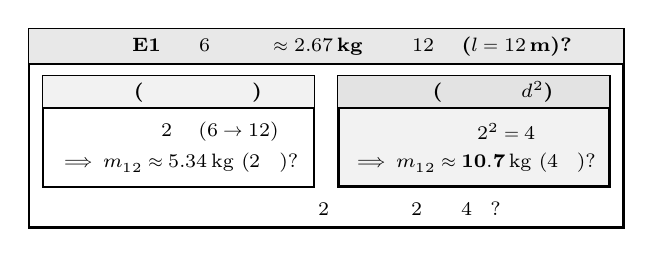
\begin{tikzpicture}[x=1cm, y=1cm, every node/.style={font=\scriptsize, text=black}]
  \draw[black, line width=0.9pt] (0,0) rectangle (7.55,2.52);
  \fill[gray!18] (0,2.08) rectangle (7.55,2.52);
  \draw[black, line width=0.6pt] (0,2.08) -- (7.55,2.08);
  \node at (3.775,2.30) {\textbf{បេសកកម្ម \en{E1}៖ ដែក $6$ លី ធ្ងន់ $\approx 2.67\unit{kg}$ ចុះដែក $12$ លី ($l = 12\unit{m}$)?}};

  % Left: Builder A (Linear misconception)
  \draw[black, line width=0.8pt] (0.18,0.52) rectangle (3.62,1.92);
  \fill[gray!10] (0.18,1.52) rectangle (3.62,1.92);
  \draw[black, line width=0.5pt] (0.18,1.52) -- (3.62,1.52);
  \node at (1.90,1.72) {\textbf{ជាង ក (គិតតាមប្រវែងលីនេអ៊ែរ)}};
  \node at (1.90,1.22) {អង្កត់ផ្ចិតកើន $2$ ដង ($6 \to 12$)};
  \node at (1.90,0.82) {$\implies m_{12} \approx 5.34\unit{kg}$ ($2$ ដង)?};

  % Right: Builder B (Quadratic cross-section truth)
  \draw[black, line width=0.95pt, fill=gray!10] (3.93,0.52) rectangle (7.37,1.92);
  \fill[gray!22] (3.93,1.52) rectangle (7.37,1.92);
  \draw[black, line width=0.55pt] (3.93,1.52) -- (7.37,1.52);
  \node at (5.65,1.72) {\textbf{ជាង ខ (គិតតាមមុខកាត់ $d^2$)}};
  \node at (5.65,1.22) {ផ្ទៃមុខកាត់កើន $2^2 = 4$ ដង};
  \node at (5.65,0.82) {$\implies m_{12} \approx \mathbf{10.7\unit{kg}}$ ($4$ ដង)?};

  \node at (3.775,0.24) {\textbf{សំណួរគន្លឹះ៖} បើអង្កត់ផ្ចិតកើន $2$ ដង តើម៉ាសកើន $2$ ដង ឬ $4$ ដង?};
\end{tikzpicture}}

% ២. E2 Explore: លំហាត់គំរូទី ១ (ទំ.៤៦--៤៧ — ម៉ាសដែក 10 លី និងដែក 12 លី ប្រវែង 12 m)
\newcommand{\figRebarModelMEASFourThree}{%
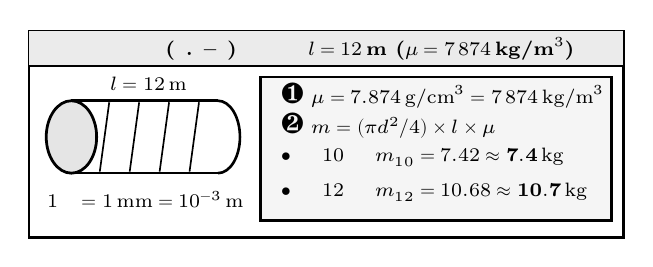
\begin{tikzpicture}[x=1cm, y=1cm, every node/.style={font=\scriptsize, text=black}]
  \draw[black, line width=0.9pt] (0,0) rectangle (7.55,2.62);
  \fill[gray!16] (0,2.18) rectangle (7.55,2.62);
  \draw[black, line width=0.6pt] (0,2.18) -- (7.55,2.18);
  \node at (3.775,2.40) {\textbf{លំហាត់គំរូទី ១ (ទំ.៤៦--៤៧)៖ ដែកប្រវែង $l = 12\unit{m}$ ($\mu = 7\,874\unit{kg/m}^3$)}};

  % Rebar rod drawing on left
  \fill[gray!20] (0.54,1.28) ellipse (0.32cm and 0.46cm);
  \draw[black, line width=0.95pt] (0.54,1.74) -- (2.40,1.74);
  \draw[black, line width=0.95pt] (0.54,0.82) -- (2.40,0.82);
  \draw[black, line width=0.95pt] (2.40,0.82) arc (-90:90:0.28cm and 0.46cm);
  \draw[black, line width=1.0pt] (0.54,1.28) ellipse (0.32cm and 0.46cm);
  \foreach \x in {0.90, 1.28, 1.66, 2.04} {
    \draw[black, line width=0.6pt] (\x,0.84) -- (\x+0.12,1.72);
  }
  \node at (1.52,1.96) {$l = 12\unit{m}$};
  \node at (1.48,0.48) {$1\text{ លី} = 1\unit{mm} = 10^{-3}\unit{m}$};

  % Calculation summary on right
  \draw[black, line width=0.8pt, fill=gray!8] (2.94,0.22) rectangle (7.40,2.04);
  \node[anchor=west] at (3.08,1.80) {\cnum{1} $\mu = 7.874\unit{g/cm}^3 = 7\,874\unit{kg/m}^3$};
  \node[anchor=west] at (3.08,1.42) {\cnum{2} $m = (\pi d^2 / 4)\times l\times \mu$};
  \node[anchor=west] at (3.08,1.02) {$\bullet$ ដែក $10$ លី៖ $m_{10} = 7.42 \approx \mathbf{7.4\unit{kg}}$};
  \node[anchor=west] at (3.08,0.58) {$\bullet$ ដែក $12$ លី៖ $m_{12} = 10.68 \approx \mathbf{10.7\unit{kg}}$};
\end{tikzpicture}}

% ៣. E3 Explain: ស្ពានបំប្លែងខ្នាតសមាស g/cm^3 -> kg/m^3 និងរូបមន្តម៉ាសមាឌ
\newcommand{\figDensityBridgeMEASFourThree}{%
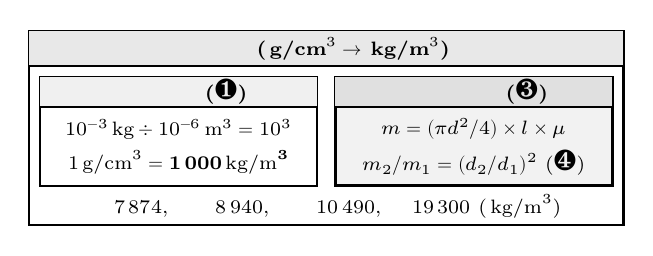
\begin{tikzpicture}[x=1cm, y=1cm, every node/.style={font=\scriptsize, text=black}]
  \draw[black, line width=0.9pt] (0,0) rectangle (7.55,2.46);
  \fill[gray!18] (0,2.02) rectangle (7.55,2.46);
  \draw[black, line width=0.6pt] (0,2.02) -- (7.55,2.02);
  \node at (3.775,2.24) {\textbf{ស្ពានបំប្លែងខ្នាតម៉ាសមាឌ ($\unit{g/cm}^3 \to \unit{kg/m}^3$) និងម៉ាសស៊ីឡាំង}};

  % Left box: Unit bridge
  \draw[black, line width=0.8pt] (0.14,0.50) rectangle (3.66,1.88);
  \fill[gray!12] (0.14,1.50) rectangle (3.66,1.88);
  \draw[black, line width=0.55pt] (0.14,1.50) -- (3.66,1.50);
  \node at (1.90,1.69) {\textbf{បំប្លែងខ្នាតសមាស (\cnum{1})}};
  \node at (1.90,1.22) {$10^{-3}\unit{kg} \div 10^{-6}\unit{m}^3 = 10^3$};
  \node at (1.90,0.80) {$1\unit{g/cm}^3 = \mathbf{1\,000\unit{kg/m}^3}$};

  % Right box: Mass formula
  \draw[black, line width=0.95pt, fill=gray!10] (3.89,0.50) rectangle (7.41,1.88);
  \fill[gray!24] (3.89,1.50) rectangle (7.41,1.88);
  \draw[black, line width=0.6pt] (3.89,1.50) -- (7.41,1.50);
  \node at (5.65,1.69) {\textbf{រូបមន្តម៉ាសដែកសរសៃ (\cnum{3})}};
  \node at (5.65,1.22) {$m = (\pi d^2 / 4)\times l\times \mu$};
  \node at (5.65,0.80) {$m_2 / m_1 = (d_2 / d_1)^2$ (\cnum{4})};

  \node at (3.775,0.24) {ដែក $7\,874$, ស្ពាន់ $8\,940$, ប្រាក់ $10\,490$, មាស $19\,300$ ($\unit{kg/m}^3$)};
\end{tikzpicture}}

% ៤. E4 Elaborate: ដែក 14 លី (ទំ.៤៧) និងលំហាត់គំរូទី ២ មាឌដែក 12 លី (ទំ.៤៧--៤៨)
\newcommand{\figVolumeMassMEASFourThree}{%
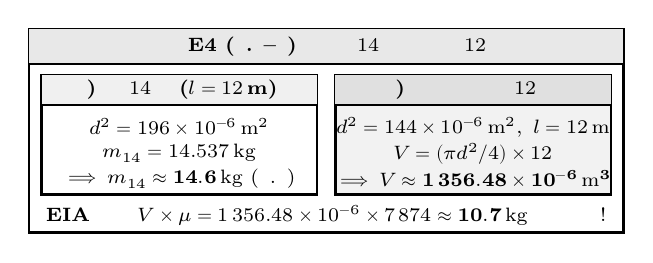
\begin{tikzpicture}[x=1cm, y=1cm, every node/.style={font=\scriptsize, text=black}]
  \draw[black, line width=0.9pt] (0,0) rectangle (7.55,2.58);
  \fill[gray!18] (0,2.14) rectangle (7.55,2.58);
  \draw[black, line width=0.6pt] (0,2.14) -- (7.55,2.14);
  \node at (3.775,2.36) {\textbf{ពង្រីក \en{E4} (ទំ.៤៧--៤៨)៖ ម៉ាសដែក $14$ លី និងមាឌដែក $12$ លី}};

  \draw[black, line width=0.8pt] (0.16,0.48) rectangle (3.66,2.00);
  \fill[gray!12] (0.16,1.62) rectangle (3.66,2.00);
  \draw[black, line width=0.55pt] (0.16,1.62) -- (3.66,1.62);
  \node at (1.91,1.81) {\textbf{១) ដែក $14$ លី ($l = 12\unit{m}$)}};
  \node at (1.91,1.34) {$d^2 = 196\times 10^{-6}\unit{m}^2$};
  \node at (1.91,1.00) {$m_{14} = 14.537\unit{kg}$};
  \node at (1.91,0.68) {$\implies m_{14} \approx \mathbf{14.6\unit{kg}}$ (ទំ.៤៧)};

  \draw[black, line width=0.95pt, fill=gray!10] (3.89,0.48) rectangle (7.39,2.00);
  \fill[gray!24] (3.89,1.62) rectangle (7.39,2.00);
  \draw[black, line width=0.6pt] (3.89,1.62) -- (7.39,1.62);
  \node at (5.64,1.81) {\textbf{២) គំរូទី ២៖ មាឌដែក $12$ លី}};
  \node at (5.64,1.34) {$d^2 = 144\times 10^{-6}\unit{m}^2, \ l = 12\unit{m}$};
  \node at (5.64,1.00) {$V = (\pi d^2 / 4)\times 12$};
  \node at (5.64,0.68) {$\implies V \approx \mathbf{1\,356.48\times 10^{-6}\unit{m}^3}$};

  \node at (3.775,0.22) {\textbf{\en{EIA}៖} ផ្ទៀង $V\times \mu = 1\,356.48\times 10^{-6}\times 7\,874 \approx \mathbf{10.7\unit{kg}}$ ត្រូវគ្នាគត់!};
\end{tikzpicture}}

% ៥. E5 Evaluate: ជម្រើសវិនិច្ឆ័យ A-D (ដុំមាសមានមាឌ V = 100 cm^3 = 10^{-4} m^3, \mu = 19.3 g/cm^3 គិតម៉ាសជា kg)
\newcommand{\figExitMEASFourThree}{%
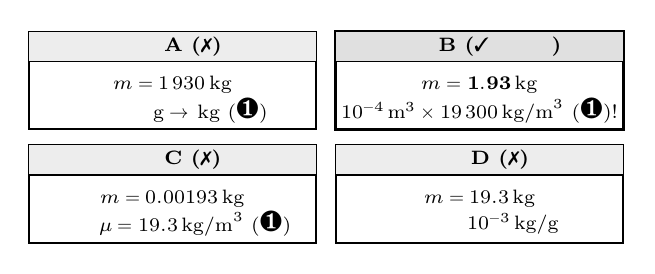
\begin{tikzpicture}[x=1cm, y=1cm, every node/.style={font=\scriptsize, text=black}]
  % Choice A
  \draw[black, line width=0.8pt] (0,1.44) rectangle (3.65,2.68);
  \fill[gray!14] (0,2.30) rectangle (3.65,2.68);
  \draw[black, line width=0.5pt] (0,2.30) -- (3.65,2.30);
  \node at (1.825,2.49) {\textbf{ជម្រើស \en{A} (\ding{55})}};
  \node at (1.825,2.00) {$m = 1\,930\unit{kg}$};
  \node at (1.825,1.68) {ភ្លេចបំប្លែង $\unit{g} \to \unit{kg}$ (\cnum{1})};

  % Choice B (Correct)
  \draw[black, line width=1.05pt] (3.90,1.44) rectangle (7.55,2.68);
  \fill[gray!24] (3.90,2.30) rectangle (7.55,2.68);
  \draw[black, line width=0.6pt] (3.90,2.30) -- (7.55,2.30);
  \node at (5.725,2.49) {\textbf{ជម្រើស \en{B} (\ding{51} ត្រឹមត្រូវ)}};
  \node at (5.725,2.00) {$m = \mathbf{1.93\unit{kg}}$};
  \node at (5.725,1.68) {$10^{-4}\unit{m}^3\times 19\,300\unit{kg/m}^3$ (\cnum{1})!};

  % Choice C
  \draw[black, line width=0.8pt] (0,0) rectangle (3.65,1.24);
  \fill[gray!14] (0,0.86) rectangle (3.65,1.24);
  \draw[black, line width=0.5pt] (0,0.86) -- (3.65,0.86);
  \node at (1.825,1.05) {\textbf{ជម្រើស \en{C} (\ding{55})}};
  \node at (1.825,0.56) {$m = 0.00193\unit{kg}$};
  \node at (1.825,0.24) {ច្រឡំថា $\mu = 19.3\unit{kg/m}^3$ (\cnum{1})};

  % Choice D
  \draw[black, line width=0.8pt] (3.90,0) rectangle (7.55,1.24);
  \fill[gray!14] (3.90,0.86) rectangle (7.55,1.24);
  \draw[black, line width=0.5pt] (3.90,0.86) -- (7.55,0.86);
  \node at (5.725,1.05) {\textbf{ជម្រើស \en{D} (\ding{55})}};
  \node at (5.725,0.56) {$m = 19.3\unit{kg}$};
  \node at (5.725,0.24) {ភ្លេចគុណនឹង $10^{-3}\unit{kg/g}$};
\end{tikzpicture}}

\begin{document}
\fontsize{10pt}{15.2pt}\selectfont

% ============================================================================
% ក្បាលរដ្ឋបាល (Administrative Header — តាមគំរូ ls_plan.tex)
% ============================================================================
{\centering
  {\muol\fontsize{11pt}{16pt}\selectfont ព្រះរាជាណាចក្រកម្ពុជា\par}
  {\muol\fontsize{11pt}{16pt}\selectfont ជាតិ សាសនា ព្រះមហាក្សត្រ\par}
  \vspace{-3pt}{\khmflourish\par}
}

\vspace{1pt}
{\muol\fontsize{10pt}{15.5pt}\selectfont
មន្ទីរអប់រំ យុវជន និងកីឡា ខេត្តកំពង់ធំ\par
ការិយាល័យអប់រំ យុវជន និងកីឡា ស្រុកកំពង់ស្វាយ\par
អនុវិទ្យាល័យព្រះក្រសាំង\par}

\vspace{2pt}
{\centering{\muol\fontsize{11.5pt}{17pt}\selectfont កិច្ចតែងការបង្រៀន\par}}
\vspace{2pt}

% --- ព័ត៌មានទូទៅ ---
{\hspace*{2.8cm}\renewcommand{\arraystretch}{1.08}
\begin{tabular}{@{}l@{\hspace{0.35cm}}p{2.9cm}@{\hspace{0.15cm}}c@{\hspace{0.25cm}}l@{}}
  - & មុខវិជ្ជា & : & គណិតវិទ្យា ថ្នាក់ទី៨ (ពីជគណិត) \\
  - & ចំណងជើងមេរៀន & : & មេរៀនទី៤៖ រង្វាស់រង្វាល់ \\
  - & ចំណងជើងរង & : & ៣. ម៉ាសធៀបនឹងមាឌ (ទំ.៤៦--៤៨, ៥០) \\
  - & រយៈពេល & : & ១ ម៉ោងសិក្សា (៥០ នាទី) \\
  - & បង្រៀនដោយ & : & ហុក ប៊ុនថែន \\
  - & កាលបរិច្ឆេទ & : & ថ្ងៃពុធ ទី២ ខែធ្នូ ឆ្នាំ២០២៦ \\
\end{tabular}\par}

\vspace{2pt}

% --- I. វត្ថុបំណង ---
{\muol\fontsize{10pt}{15.5pt}\selectfont \enbf{I.} វត្ថុបំណង\par}
\vspace{1pt}
{\renewcommand{\arraystretch}{1.10}
\begin{tabular}{@{}p{0.55cm}@{}p{2.35cm}@{\hspace{0.15cm}}c@{\hspace{0.25cm}}p{14.95cm}@{}}
  \hfill\wcirc\hspace{0.2cm} & វិជ្ជាសម្បទា & : & សិស្សប្រាប់និយមន័យម៉ាសធៀបនឹងមាឌ (ម៉ាសមាឌ $\mu$) ការបំប្លែងខ្នាត $1\unit{g/cm}^3 = 1\,000\unit{kg/m}^3$ ពាក្យសំណង់ «ដែកលី» ($1\text{ លី} = 1\unit{mm}$) និងរូបមន្តម៉ាសសរសៃដែករាងស៊ីឡាំង $m = V\times \mu = (\pi d^2 / 4)\times l\times \mu$ បានត្រឹមត្រូវ ។ \\
  \hfill\wcirc\hspace{0.2cm} & បំណិនសម្បទា & : & សិស្សគណនាម៉ាសជា $\unit{kg}$ មាឌជា $\unit{m}^3$ និងប្រាក់ចំណាយទិញសរសៃដែកសំណង់ (ដែក $6$ លី, $10$ លី, $12$ លី, $14$ លី) ព្រមទាំងខ្សែភ្លើងស្ពាន់លើសន្លឹកកិច្ចការ (ទំ.៤៦--៤៨, ៥០) បានត្រឹមត្រូវ ។ \\
  \hfill\wcirc\hspace{0.2cm} & ចរិយាសម្បទា & : & សិស្សមានទម្លាប់គណនាទម្ងន់និងថ្លៃដែកសំណង់តាមរូបមន្តវិទ្យាសាស្ត្រច្បាស់លាស់ ជៀសវាងការប៉ាន់ស្មានខុសក្នុងការងារសាងសង់ជាក់ស្ដែង ។ \\
\end{tabular}\par}

\vspace{2pt}

% --- II. សម្ភារៈឧបទេស ---
{\muol\fontsize{10pt}{15.5pt}\selectfont \enbf{II.} សម្ភារៈឧបទេស\par}
\vspace{1pt}
\hspace*{0.55cm}$\bullet$\ សៀវភៅសិក្សាគោលថ្នាក់ទី៨ (ទំ.៤៦--៤៨, ៥០) ក្ដារខៀន ដីស/ហ្វឺត បន្ទាត់ត្រង់ និង\textbf{សន្លឹកកិច្ចការសិស្សបំពេញចន្លោះ ស-ខ្មៅ} (\en{Printable\_Materials\_MEAS43} ទំព័រ ១--២ សម្រាប់សិស្ស និងទំព័រ ៣ ប្លង់ក្ដារខៀន/ចម្លើយគ្រូ — គ្មានប្រើ \en{LCD})\par

\vspace{2pt}

% --- III. វិធីសាស្រ្តបង្រៀន ---
{\muol\fontsize{10pt}{15.5pt}\selectfont \enbf{III.} វិធីសាស្រ្តបង្រៀន\par}
\vspace{1pt}
{\renewcommand{\arraystretch}{1.08}
\begin{tabular}{@{}p{0.55cm}@{}p{2.35cm}@{\hspace{0.15cm}}c@{\hspace{0.25cm}}p{14.95cm}@{}}
  \hfill$\bullet$\hspace{0.2cm} & គោលវិធី & : & សិស្សមជ្ឈមណ្ឌល (សន្លឹកកិច្ចការបំពេញចន្លោះជាគោល + ការពិភាក្សាជាក្រុមតូច ៣ នាក់) \\
  \hfill$\bullet$\hspace{0.2cm} & យុទ្ធវិធីបង្រៀន & : & គំរូស្ថាបនានិយម \en{5Es} រួមបញ្ចូល \textbf{ស្ពានបំប្លែងខ្នាតសមាស $\unit{g/cm}^3 \to \unit{kg/m}^3$} និង \textbf{ការបំបែកអន្ទាក់សមាមាត្រលីនេអ៊ែរលើអង្កត់ផ្ចិត $d^2$} \\
\end{tabular}\par}

\vspace{2pt}

% --- IV. ដំណើរការបង្រៀន ---
{\muol\fontsize{10pt}{15.5pt}\selectfont \enbf{IV.} ដំណើរការបង្រៀន\par}

{\renewcommand{\arraystretch}{1.15}
\begin{longtable}{|L{5.50cm}|L{7.90cm}|L{4.80cm}|}
\hline
\multicolumn{1}{|c|}{\cellcolor{headgray}\muol សកម្មភាពគ្រូ} &
\multicolumn{1}{c|}{\cellcolor{headgray}\muol ខ្លឹមសារមេរៀន} &
\multicolumn{1}{c|}{\cellcolor{headgray}\muol សកម្មភាពសិស្ស} \\
\hline
\endfirsthead

\hline
\multicolumn{1}{|c|}{\cellcolor{headgray}\muol សកម្មភាពគ្រូ} &
\multicolumn{1}{c|}{\cellcolor{headgray}\muol ខ្លឹមសារមេរៀន} &
\multicolumn{1}{c|}{\cellcolor{headgray}\muol សកម្មភាពសិស្ស} \\
\hline
\endhead

% ==================== ជំហានទី១ (2min) ====================
\stepheader{ជំហានទី១ \enbf{(}រដ្ឋបាលថ្នាក់\enbf{)}}
$\bullet$ ពិនិត្យវត្តមាន អនាម័យ និងសណ្ដាប់ធ្នាប់ថ្នាក់រៀន \par
$\bullet$ រៀបចំក្រុមតូច ៣ នាក់តាមតុ និងចែក\textbf{សន្លឹកកិច្ចការសិស្ស (\en{MEAS43} ទំព័រ ១–២)}
&
$\bullet$ រដ្ឋបាលថ្នាក់ អនាម័យ និងវិន័យសិក្សា \par
$\bullet$ ចែកសន្លឹកកិច្ចការម្នាក់ ១ សន្លឹក សម្រាប់បំពេញតាមដំណាក់កាល \en{E1--E5}
&
$\circ$ ប្រធានថ្នាក់រាយការណ៍វត្តមានសិស្ស \par
$\circ$ ទទួលសន្លឹកកិច្ចការ សរសេរឈ្មោះ និងអង្គុយតាមក្រុម ៣ នាក់ \\
\hline

% ==================== ជំហានទី២ (9min: កំណែ <=3m + រំលឹក 3m + E1 3m) ====================
\stepheader{ជំហានទី២ \enbf{(}កិច្ចការផ្ទះ \enbf{+} ទំនាក់ទំនងមេរៀនថ្មី\enbf{)}}
\ditem \textbf{កំណែកិច្ចការផ្ទះ ($\le\text{\enbf{3\,min}}$)} \par
$\bullet$ ហៅសិស្ស ២ នាក់ឡើងកែលំហាត់ទំ.៥០ លេខ ៥ (ក និង ខ) លើក្ដារខៀន
&
{\centering\redsub{កំណែកិច្ចការផ្ទះមេរៀនមុន (ទំ.៥០ \#5 ក និង ខ)}\par}
$\bullet$ \textbf{\#5 (សៀវភៅ $100$ ទំព័រ $= 50$ សន្លឹក $+ 2$ ក្រប, $S_1 = 0.03108\unit{m}^2$, $10\,000$ ក្បាល, ខាត $4\%$)៖} \par
\hspace*{0.2cm}-- ម៉ាសសុទ្ធ ១ ក្បាល $= 0.118104\unit{kg}$ $\implies$ \textbf{(ក)} ម៉ាសសរុប $= \mathbf{1\,228.28\unit{kg}}$ \par
\hspace*{0.2cm}-- \textbf{(ខ)} ថ្លៃក្រដាស ១ ក្បាល $= 0.122828\times 4\,800 \approx \mathbf{590\riel}$
&
$\circ$ ផ្ទៀងចម្លើយ និងកែតម្រូវចូលសៀវភៅកិច្ចការផ្ទះ \\[3pt]

\ditem \textbf{រំលឹកមេរៀនទាក់ទង (\enbf{3min})} \par
$\bullet$ សួរ៖ «តើ $1\unit{cm}^3$ ស្មើប៉ុន្មាន $\unit{m}^3$? ចុះ $10^{-3}\div 10^{-6}$ ស្មើប៉ុន្មាន?»
&
{\centering\redsub{រំលឹកមាឌគូប $1\unit{cm}^3$ និងប្រភាគស្វ័យគុណគោល $10$}\par}
$\bullet$ បំប្លែងមាឌ៖ $1\unit{cm}^3 = (10^{-2}\unit{m})^3 = 10^{-6}\unit{m}^3$ និង $\tfrac{10^{-3}}{10^{-6}} = 10^3 = 1\,000$
&
$\circ$ ឆ្លើយ៖ «$1\unit{cm}^3 = 10^{-6}\unit{m}^3$ ហើយផលចែកស្មើ $1\,000$!» \\[3pt]

$\bullet$ សួរបន្ត៖ «ចុះមាឌសរសៃដែករាងស៊ីឡាំងដែលមានអង្កត់ផ្ចិត $d$ និងប្រវែង $l$ ស្មើអ្វី?»
&
$\bullet$ មាឌស៊ីឡាំង៖ $V = S\times l = \dfrac{\pi d^2}{4}\times l$ ($\pi \approx 3.14$)
&
$\circ$ ឆ្លើយ៖ «$V = \frac{\pi d^2}{4}\times l$!» \\[3pt]

\fiveE{E1 - Engage (3min)} \timenote{(កុំទាន់ផ្ដល់ចម្លើយ)} \par
\ditem \textbf{បេសកកម្មជាងសំណង់ស្ទង់ទម្ងន់ដែកសរសៃ (សន្លឹកកិច្ចការ \en{E1})} \par
$\bullet$ ឱ្យសិស្សអានប្រអប់ \en{E1} ហើយគូសជ្រើសរើសរវាង\textbf{ជាង ក} និង\textbf{ជាង ខ}
&
\redsub{បេសកកម្ម \en{E1}៖ ដែក $6$ លី ($d = 6\unit{mm}$) មួយដើមប្រវែង $12\unit{m}$ ធ្ងន់ $\approx 2.67\unit{kg}$} \par
ចុះបើលើក\textbf{ដែក $12$ លី} ($d = 12\unit{mm}$ អង្កត់ផ្ចិតធំជាងមុន $2$ ដង ប្រវែង $12\unit{m}$ ដូចគ្នា)៖ \par
$\bullet$ \textbf{ជាង ក} ថាធ្ងន់ $2$ ដង ($\approx 5.34\unit{kg}$) ឯ\textbf{ជាង ខ} ថាធ្ងន់ $4$ ដង ($\approx 10.7\unit{kg}$)! តើអ្នកណាត្រូវ?
&
$\circ$ ពិភាក្សាជាគូ និងគូស \ding{51} ក្នុងប្រអប់ \en{E1} លើសន្លឹកកិច្ចការ \\[3pt]

&
\cfig{\figEngageMEASFourThree}
& \\
\hline

% ==================== ជំហានទី៣ (17min: E2 11m + E3 6m) ====================
\stepheader{ជំហានទី៣ \enbf{(}ខ្លឹមសារមេរៀនថ្មី\enbf{)}}
\fiveE{E2 - Explore (11min)} \par
$\bullet$ សរសេរចំណងជើងរង \textbf{៣. ម៉ាសធៀបនឹងមាឌ} លើក្ដារខៀន \par
\ditem \textbf{សកម្មភាព ១៖ ម៉ាសមាឌ និងលំហាត់គំរូទី ១ — ដែក $10$ លី និង $12$ លី (\enbf{6min}, \en{E2-A})} \par
$\bullet$ ណែនាំម៉ាសមាឌលោហធាតុ និងពាក្យ «ដែកលី» (ទំ.៤៦) រួចឱ្យសិស្សបំពេញជំហានគណនា $m_{10}, m_{12}$
&
មេរៀនទី៤ \quad {\muol រង្វាស់រង្វាល់ \enbf{(}ត\enbf{)}} \par
៣. ម៉ាសធៀបនឹងមាឌ \par
$\bullet$ វត្ថុធ្ងន់ដូចជាលោហធាតុ គេគិតម៉ាសធៀបនឹងមាឌ ហៅថា \textbf{ម៉ាសមាឌ ($\mu$)}៖ ដែក $7.874\unit{g/cm}^3$, ស្ពាន់ $8.94\unit{g/cm}^3$, ប្រាក់ $10.49\unit{g/cm}^3$, មាស $19.3\unit{g/cm}^3$ \par
$\bullet$ \textbf{សម្គាល់ (ទំ.៤៦)៖} ដែកអង្កត់ផ្ចិត $6\unit{mm}$ ហៅថា \textbf{ដែក $6$ លី} ($1\text{ លី} = 1\unit{mm} = 10^{-3}\unit{m}$) \par
$\bullet$ \textbf{បំប្លែងម៉ាសមាឌដែក៖} $\mu = \dfrac{7.874\times 10^{-3}\unit{kg}}{(10^{-2}\unit{m})^3} = \mathbf{7\,874\unit{kg/m}^3}$
&
$\circ$ កត់សម្គាល់ពាក្យ «ដែកលី» និងបំប្លែងឃើញ $\mu = 7\,874\unit{kg/m}^3$ \\[3pt]

$\bullet$ ឱ្យសិស្សគណនាម៉ាសដែក $10$ លី និងដែក $12$ លី ($l = 12\unit{m}$) លើសន្លឹកកិច្ចការ \en{E2-A}
&
$\bullet$ \textbf{លំហាត់គំរូទី ១ (ទំ.៤៦–៤៧ — ដែកមួយដើម $l = 12\unit{m}, \mu = 7\,874\unit{kg/m}^3, \pi = 3.14$)៖} \par
\hspace*{0.2cm}-- \textbf{ដែក $10$ លី} ($d^2 = 100\times 10^{-6}\unit{m}^2$)៖ $m_{10} = 3.14\times \dfrac{100\times 10^{-6}}{4}\times 12\times 7\,874 = 7.4173 \approx \mathbf{7.4\unit{kg}}$ \par
\hspace*{0.2cm}-- \textbf{ដែក $12$ លី} ($d^2 = 144\times 10^{-6}\unit{m}^2$)៖ $m_{12} = 3.14\times \dfrac{144\times 10^{-6}}{4}\times 12\times 7\,874 = 10.680 \approx \mathbf{10.7\unit{kg}}$
&
$\circ$ គណនាឃើញដែក $10$ លី $\approx 7.4\unit{kg}$ និងដែក $12$ លី $\approx 10.7\unit{kg}$ \\[3pt]

&
\cfig{\figRebarModelMEASFourThree}
& \\[3pt]

\ditem \textbf{សកម្មភាព ២៖ អន្ទាក់បំប្លែង $\unit{g/cm}^3 \to \unit{kg/m}^3$ និងផលធៀប $d^2$ (\enbf{5min}, \en{E2-B})} \par
$\bullet$ សួរ៖ «ហេតុអ្វីប្ដូរពី $\unit{g/cm}^3$ ទៅ $\unit{kg/m}^3$ ត្រូវគុណនឹង $1\,000$ មិនមែនចែកនឹង $1\,000$?»
&
$\bullet$ \textbf{ពិនិត្យអន្ទាក់ទី ១ (ខ្នាតសមាស)៖} \par
\hspace*{0.2cm}ក្នុង $1\unit{m}^3$ មានដល់ទៅ $1\,000\,000\unit{cm}^3$ ដូច្នេះដែក $1\unit{m}^3$ ធ្ងន់ដល់ទៅ $7\,874\unit{kg}$ ($\approx 7.87\text{ តោន}$)!
&
$\circ$ រកឃើញថា $1\unit{g/cm}^3 = 1\,000\unit{kg/m}^3$ \\[3pt]

$\bullet$ សួរបន្ត៖ «ចុះធៀបនឹងដែក $6$ លី ($2.67\unit{kg}$) តើដែក $12$ លី ($10.68\unit{kg}$) ធ្ងន់ជាងប៉ុន្មានដង?»
&
$\bullet$ \textbf{ពិនិត្យអន្ទាក់ទី ២ (ការេអង្កត់ផ្ចិត $d^2$)៖} \par
\hspace*{0.2cm}ដែក $12$ លី ($10.68\unit{kg}$) ធ្ងន់ជាងដែក $6$ លី ($2.67\unit{kg}$) ចំនួន $\mathbf{4}$ ដង ព្រោះ $(12/6)^2 = 4$!
&
$\circ$ រកឃើញថាម៉ាសដែកសមាមាត្រនឹងការេអង្កត់ផ្ចិត $d^2$ \\[3pt]

% --- E3 Explain (6min) ---
\fiveE{E3 - Explain (6min)} \par
$\bullet$ ដឹកនាំសិស្សសង្ខេបរូបមន្ត\textbf{ម៉ាសធៀបនឹងមាឌ (ម៉ាសមាឌ $\mu$)} និងម៉ាសស៊ីឡាំង (ទំ.៤៦–៤៧)
&
$\bullet$ \textbf{ក្បួនគណនាម៉ាសធៀបនឹងមាឌ (ទំ.៤៦–៤៨)៖} \par
\hspace*{0.15cm}១) បំប្លែងខ្នាត៖ \graybox{$1\unit{g/cm}^3 = 1\,000\unit{kg/m}^3$} \quad ២) ម៉ាសវត្ថុ៖ \graybox{$m = V\times \mu$}
&
$\circ$ បំពេញប្រអប់រូបមន្តលើសន្លឹកកិច្ចការ \en{E3} \\[3pt]

$\bullet$ កត់ត្រារូបមន្តម៉ាសសរសៃដែករាងស៊ីឡាំង និងផលធៀបម៉ាសតាមអង្កត់ផ្ចិត
&
\hspace*{0.15cm}៣) សរសៃដែកស៊ីឡាំង៖ \graybox{$m = \dfrac{\pi d^2}{4}\times l\times \mu$} \quad ៤) ប្រវែងនិងលោហៈដូចគ្នា៖ \graybox{$\dfrac{m_2}{m_1} = \left(\dfrac{d_2}{d_1}\right)^2$}
&
$\circ$ កត់ត្រារូបមន្ត $m$ និងផលធៀប $d^2$ លើសន្លឹកកិច្ចការ \en{E3} \\[3pt]

&
\cfig{\figDensityBridgeMEASFourThree}
& \\[3pt]

$\bullet$ ភ្ជាប់\textbf{ធនាគារហេតុផល \cnum{1}--\cnum{4}} លើក្ដារខៀន និងសន្លឹកកិច្ចការ
&
\textbf{ធនាគារហេតុផល (\en{Warrant Bank})៖} \par
\cnum{1} \textbf{ម៉ាសមាឌជា $\unit{kg/m}^3$៖} $1\unit{g/cm}^3 = 1\,000\unit{kg/m}^3$ (ដែក $\mu = 7\,874\unit{kg/m}^3$, ស្ពាន់ $\mu = 8\,940\unit{kg/m}^3$) \par
\cnum{2} \textbf{ខ្នាតដែកលី៖} ដែក $k$ លី $\iff d = k\unit{mm} = k\times 10^{-3}\unit{m} \implies d^2 = k^2\times 10^{-6}\unit{m}^2$ \par
\cnum{3} \textbf{ម៉ាសសរសៃដែក/ខ្សែស្ពាន់៖} $m = V\times \mu = \frac{\pi d^2}{4}\times l\times \mu$ ($V$ ជា $\unit{m}^3, \mu$ ជា $\unit{kg/m}^3 \implies m$ ជា $\unit{kg}$) \par
\cnum{4} \textbf{ផលធៀបតាមការេអង្កត់ផ្ចិត៖} បើ $l$ និង $\mu$ ដូចគ្នា នោះ $m_2 = m_1 \times \left(\frac{d_2}{d_1}\right)^2$
&
$\circ$ ផ្ទៀងលេខកូដ \cnum{1}--\cnum{4} លើសន្លឹកកិច្ចការ \\
\hline

% ==================== ជំហានទី៤ (20min: E4 10m + E5 10m) ====================
\stepheader{ជំហានទី៤ \enbf{(}ពង្រីកចំណេះដឹង\enbf{)}}
\fiveE{E4 - Elaborate (10min)} \par
\ditem \textbf{ម៉ាសដែក $14$ លី (ទំ.៤៧) និងលំហាត់គំរូទី ២៖ មាឌដែក $12$ លី (ទំ.៤៧–៤៨)} \par
$\bullet$ ឱ្យសិស្សគណនាម៉ាសដែក $14$ លី និងមាឌដែក $12$ លី គិតជា $\unit{m}^3$ លើសន្លឹកកិច្ចការ \en{E4}
&
{\muol ពង្រីកគំរូទី ១ និង លំហាត់គំរូទី ២} \textbf{(ទំ.៤៧–៤៨, $l = 12\unit{m}, \pi = 3.14$)៖} \par
$\bullet$ \textbf{១) ម៉ាសដែក $14$ លី} ($d = 14\times 10^{-3}\unit{m} \implies d^2 = 196\times 10^{-6}\unit{m}^2$)៖ \par
\hspace*{0.2cm}$m_{14} = 3.14\times \dfrac{196\times 10^{-6}}{4}\times 12\times 7\,874 = 14.537\unit{kg} \approx \graybox{$14.6\unit{kg}$}$ (តាមសៀវភៅគោលទំ.៤៧) \par
$\bullet$ \textbf{២) លំហាត់គំរូទី ២ (មាឌដែក $12$ លី មួយដើមគិតជា $\unit{m}^3$)៖} \par
\hspace*{0.2cm}$V = \dfrac{\pi d^2}{4}\times l = \dfrac{3.14\times 144\times 10^{-6}}{4}\times 12 \approx \graybox{$1\,356.48\times 10^{-6}\unit{m}^3$}$ (\cnum{2})
&
$\circ$ គណនាឃើញ $m_{14} \approx 14.6\unit{kg}$ និងមាឌដែក $12$ លី $V \approx 1\,356.48\times 10^{-6}\unit{m}^3$ \\[3pt]

&
\cfig{\figVolumeMassMEASFourThree}
& \\[3pt]

$\bullet$ សួរសំណួរឆ្លុះបញ្ចាំង \textbf{\en{EIA Looking-Back} (1min)}
&
\textbf{\en{EIA Looking-Back}៖} «បើយកមាឌដែក $12$ លី $V = 1\,356.48\times 10^{-6}\unit{m}^3$ ទៅគុណនឹង $\mu = 7\,874\unit{kg/m}^3$ តើឃើញប៉ុន្មាន $\unit{kg}$?» ($\to 10.68\unit{kg} \approx 10.7\unit{kg}$ ត្រូវគ្នា ១០០\% នឹងគំរូទី ១!)
&
$\circ$ ផ្ទៀងផ្ទាត់ឃើញ $V\times \mu \approx 10.7\unit{kg}$ ស៊ីចង្វាក់គ្នាឥតខ្ចោះ \\[3pt]

% --- E5 Evaluate (10min) ---
\fiveE{E5 - Evaluate (10min)} \par
\ditem \textbf{ប្រតិបត្តិជាក្រុមតូច ៣ នាក់ (4min, សន្លឹកកិច្ចការ \en{E5})} \par
$\bullet$ ឱ្យសិស្សគណនាម៉ាសដែក $6$ លី ($200$ ដើម) និងដែក $10$ លី ($20$ ដើម) ក្នុងលំហាត់ប្រតិបត្តិ (ទំ.៤៨)
&
{\muol លំហាត់ប្រតិបត្តិ} \textbf{(ទំ.៤៨ — ពូសុខទិញដែក $6$ លី $200$ ដើម និងដែក $10$ លី $20$ ដើម, $l=12\unit{m}, 2\,800\riel/\unit{kg}$)៖} \par
$\bullet$ ដែក $6$ លី ១ ដើម៖ $m_6 = 3.14\times \frac{36\times 10^{-6}}{4}\times 12\times 7\,874 \approx 2.6702\unit{kg} \implies 200$ ដើម $= 534.04\unit{kg}$ \par
$\bullet$ ដែក $10$ លី ១ ដើម៖ $m_{10} \approx 7.4173\unit{kg} \implies 20$ ដើម $= 148.35\unit{kg}$ (\cnum{3})
&
$\circ$ គណនាម៉ាសដែក $6$ លីសរុប និងដែក $10$ លីសរុប \\[3pt]

$\bullet$ ឱ្យសិស្សបូកម៉ាសដែកទាំងពីរមុខ រួចគណនាប្រាក់ដែលពូសុខត្រូវចំណាយ
&
$\bullet$ ម៉ាសសរុប $m \approx 682.39\unit{kg} \implies$ ប្រាក់ចំណាយ $\approx 682.39\times 2\,800 \approx \graybox{$1\,910\,690\riel$}$ \par
\hspace*{0.2cm}(បើគិតតាមតម្លៃបង្គត់ $m_6\approx 2.67\unit{kg}, m_{10}\approx 7.4\unit{kg}$ បាន $682\unit{kg} \implies 1\,909\,600\riel$)
&
$\circ$ គណនាជាក្រុមឃើញពូសុខចំណាយប្រហែល $1\,910\,690\riel$ \\[3pt]

$\bullet$ ឱ្យក្រុមសិស្សផ្ទៀងផ្ទាត់និង\textbf{បិទបេសកកម្ម \en{E1} (2min)}
&
$\bullet$ \textbf{បិទបេសកកម្ម \en{E1}៖} ជាង ខ ត្រឹមត្រូវ! ដែក $12$ លី ធ្ងន់ $\approx \mathbf{10.7\unit{kg}}$ (ធ្ងន់ជាងដែក $6$ លី ចំនួន $(12/6)^2 = \mathbf{4}$ ដង)!
&
$\circ$ បិទបេសកកម្ម \en{E1} ឃើញជាង ខ ត្រឹមត្រូវ ($4$ ដង) \\[3pt]

\ditem \textbf{សំណួរវិនិច្ឆ័យ \en{A--D} និងសំបុត្រចេញ (4min)} \par
$\bullet$ ឱ្យសិស្សគូសរង្វង់ជម្រើសត្រូវលើសន្លឹកកិច្ចការ រួចលើកម្រាមដៃ ១--៤
&
{\centering\textbf{សំណួរវិនិច្ឆ័យ \en{A--D}៖ ដុំមាសសុទ្ធមួយដុំមានមាឌ $V = 100\unit{cm}^3 = 10^{-4}\unit{m}^3$ ($\mu_{\text{មាស}} = 19.3\unit{g/cm}^3$) ។ តើដុំមាសនេះមានម៉ាសប៉ុន្មាន $\unit{kg}$?}\par}
&
$\circ$ វិភាគជម្រើស \en{A--D} និងលើកម្រាមដៃ ២ (\textbf{ជម្រើស \en{B}}) \\[3pt]

&
\cfig{\figExitMEASFourThree}
& \\[3pt]

$\bullet$ បញ្ជាក់ចម្លើយត្រូវ (\textbf{ជម្រើស \en{B}}) និងឱ្យបំពេញ\textbf{សំបុត្រចេញ ៦០ វិនាទី}
&
$\bullet$ \textbf{សំបុត្រចេញ៖} ម៉ាសមាឌស្ពាន់ $\mu = 8.94\unit{g/cm}^3 = \mathbf{8\,940\unit{kg/m}^3}$; បើដុំស្ពាន់មានមាឌ $V = 2\times 10^{-3}\unit{m}^3$ នោះម៉ាស $m = \mathbf{17.88\unit{kg}}$ ។
&
$\circ$ បំពេញសំបុត្រចេញលើសន្លឹកកិច្ចការមុនបញ្ចប់ម៉ោង \\
\hline

% ==================== ជំហានទី៥ (<=2min) ====================
\stepheader{ជំហានទី៥ \enbf{(}កិច្ចការផ្ទះ \enbf{+} បណ្ដាំផ្ញើ\enbf{)}}
\timenote{ចំណាយពេលឱ្យតិចបំផុតកុំឱ្យលើស 2min} \par
$\bullet$ ណែនាំប្រអប់\textbf{កិច្ចការផ្ទះ}លើសន្លឹកកិច្ចការទំព័រ ២ (លំហាត់ទំ.៥០ លេខ ៤ និង លេខ ៦)
&
{\centering{\muol កិច្ចការផ្ទះ} \textbf{(សៀវភៅគោល ទំ.៥០ លេខ ៤ និង លេខ ៦)}\par} \par
$\bullet$ \textbf{\#4 (ទំ.៥០)៖} គេដឹងថាដែក $10$ លីមួយដើមមានម៉ាស $7.4\unit{kg}$ ។ ចូររកម៉ាសនៃដែក $16$ លីវិញ ។ \par
$\bullet$ \textbf{\#6 (ទំ.៥០)៖} ខ្សែភ្លើងស្ពាន់មួយដុំប្រវែង $100\unit{m}$ អង្កត់ផ្ចិតមុខកាត់ $2\frac{1}{2}\unit{mm}$ ($= 2.5\unit{mm}$) និង $\mu = 8.94\unit{g/cm}^3$ ។ រកម៉ាសស្ពាន់ (មិនគិតជ័រស្រោប) ។
&
$\circ$ គូសចំណាំលំហាត់ \#4 និង \#6 ទំ.៥០ \\[3pt]

$\bullet$ ផ្ដាំផ្ញើឱ្យអានមុនចំណុចទី ៤ (ល្បឿនមធ្យម) សម្រាប់ម៉ោងបញ្ចប់មេរៀនទី៤
&
$\bullet$ \textbf{បណ្ដាំផ្ញើ៖} អានមុន \textbf{៤. ល្បឿនមធ្យម (ទំ.៤៨–៤៩)} និងសង្កេតខ្នាត $\unit{km/h}$ ធៀបនឹង $\unit{m/s}$ ។
&
$\circ$ កត់ត្រាបណ្ដាំផ្ញើ ទុកសន្លឹកកិច្ចការក្នុងសៀវភៅ និងជម្រាបលាគ្រូ \\
\hline
\end{longtable}}

\vspace{6pt}
% --- ហត្ថលេខា (កាលបរិច្ឆេទត្រូវគ្នា ១០០% នឹងខាងលើ) ---
{\centering
\hspace*{5.2cm}\begin{minipage}{11.5cm}
  \centering
  ថ្ងៃពុធ ៨រោច ខែកត្តិក ឆ្នាំមមី អដ្ឋស័ក ពុទ្ធសករាជ ២៥៧០\par
  កំពង់ស្វាយ, ថ្ងៃទី២ ខែធ្នូ ឆ្នាំ២០២៦\par
  \vspace{2pt}
  {\muol គ្រូបង្រៀន\par}
  \vspace{32pt}
  \hfill{\muol ហុក ប៊ុនថែន}\hspace*{1.4cm}
\end{minipage}\par}

\end{document}
